\documentclass{tufte-handout}

\title{On ultimate; O4: primary long or right-wing}
\author[James Reynolds]{James Reynolds}

%\date{28 March 2010} % without \date command, current date is supplied

%\geometry{showframe} % display margins for debugging page layout

\usepackage{graphicx} % allow embedded images
  \setkeys{Gin}{width=\linewidth,totalheight=\textheight,keepaspectratio}
  \graphicspath{{graphics/}} % set of paths to search for images
\usepackage{amsmath}  % extended mathematics
\usepackage{booktabs} % book-quality tables
\usepackage{units}    % non-stacked fractions and better unit spacing
\usepackage{multicol} % multiple column layout facilities
\usepackage{lipsum}   % filler text
\usepackage{fancyvrb} % extended verbatim environments
  \fvset{fontsize=\normalsize}% default font size for fancy-verbatim environments

% Standardize command font styles and environments
\newcommand{\doccmd}[1]{\texttt{\textbackslash#1}}% command name -- adds backslash automatically
\newcommand{\docopt}[1]{\ensuremath{\langle}\textrm{\textit{#1}}\ensuremath{\rangle}}% optional command argument
\newcommand{\docarg}[1]{\textrm{\textit{#1}}}% (required) command argument
\newcommand{\docenv}[1]{\textsf{#1}}% environment name
\newcommand{\docpkg}[1]{\texttt{#1}}% package name
\newcommand{\doccls}[1]{\texttt{#1}}% document class name
\newcommand{\docclsopt}[1]{\texttt{#1}}% document class option name
\newenvironment{docspec}{\begin{quote}\noindent}{\end{quote}}% command specification environment

\begin{document}

\maketitle% this prints the handout title, author, and date
%\printclassoptions
This is 
a two-pager 
about 
primary long and 
right wing on offence\footnote{
Referred to here 
as position O4. 
This
is part of a series, 
available at
\url{https://github.com/James-Reynolds/Ultimate-strategy-and-tactics}}. 

\section{Beating person-match defence with a vertical stack}\label{sec:vertical}

\begin{marginfigure}%
  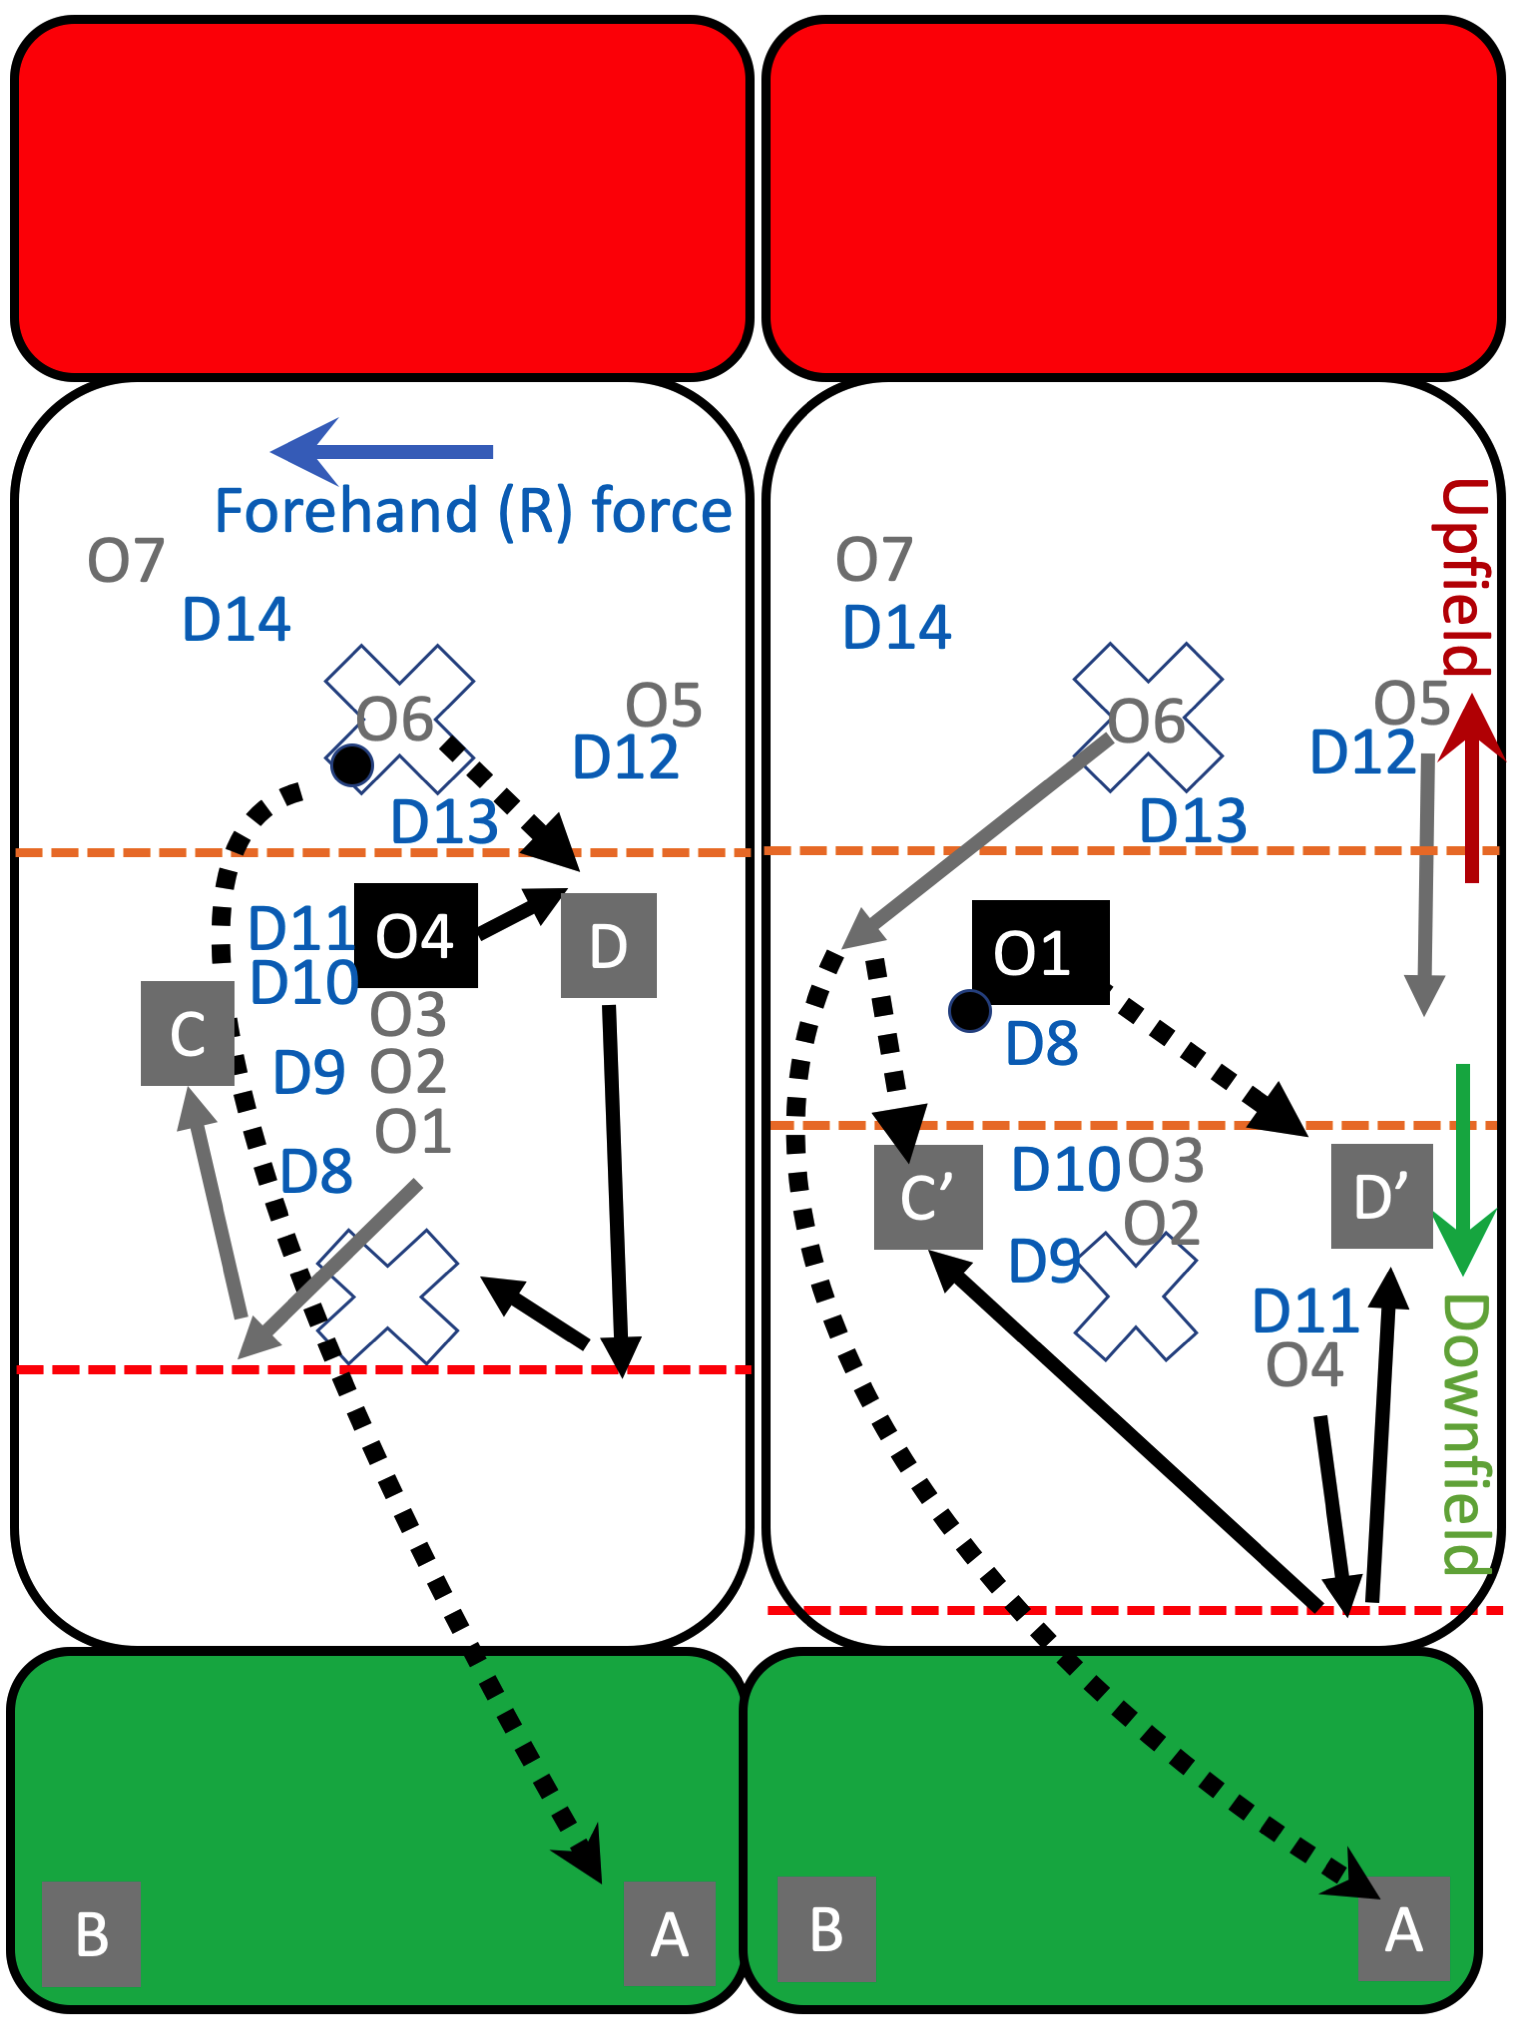
\includegraphics[width=\linewidth]{O4-vertical}
  \caption{Vertical stack: 
  starting position (left),
  and development (right)}
  \label{fig:O4-vertical}
\end{marginfigure}

Figure \ref{fig:O4-vertical} (left) shows 
a situation 
with 
your team: 
using 
a vertical stack formation; 
having called a brick; and
facing a 
forehand force with 
person-match defence\footnote{
Vertical works
against other person-match defences, 
but might need 
adjustment e.g. 
(1) backhand force,
mirror everything;
(2) straight up force, 
maybe give the handlers 
time to move the disc around, 
and go out to the sidelines
when you do cut; etc.}. 
You (O4) 
are at the front 
of the stack.
O6 might be able 
to throw you
a break
to D, 
perhaps without you
even having to cut. 
If you do cut, 
you might 
go to the break side\footnote{ 
This potentially opens 
up the field in front of 
the other cutters 
for them to cut under.} 
and then head deep towards A. 
Figure \ref{fig:O4-vertical} (left) 
shows this movement with 
solid black arrows


You 
(O4)
or any of the other cutters
(O1. O2, O4) 
might run onto 
this pass 
after it is thrown\footnote{
Note, cutting to D 
before the throw 
risks causing a pick, 
as D10 
might be obstructed
 by O4 
 or O2. 
 However, 
 if you do not move 
 until the disc is in the air
 the pass may stand,
 with any pick 
 just allowing 
 D10 to
 catch up 
 to put the force on 
 a bit earlier.}.

Otherwise, 
as secondary long, 
(O4) 
your role 
will likely 
involve cutting 
\smallcaps{after} 
the secondary middle, O2\footnote{
Starting
in the middle of the vertical stack,
as shown in 
Figure \ref{fig:O4-vertical} (left),
it is difficult for 
you to make 
an initial cut 
without causing 
a pick.}.
The play might develop 
in lots of different ways, 
but
Figure \ref{fig:O4-vertical} (right) shows 
one outcome, 
with the disc 
having gone 
to O1\footnote{
O1 has cut under 
on the open side.
O4 is indicated 
clearing 
back to the stack 
or cutting 
deep on 
the break side. 
The stack is shown having 
moved further downfield.}. 
This leaves 
you 
available 
at the front of the stack. 
You might: 
(1) stand still until O1
(or someone else)  
throws it 
to D'\footnote{
This throw 
breaks the force, 
so it is likely 
that D10 will 
be on the wrong side 
of you to make an interception.};
(2) cut to A;
or wait till O2 
cuts to C, 
then cut to (3) A,
(4) B, or 
back-under 
(dashed grey arrow) 
to (5) C'.  

O4 is called secondary long, 
because you provide the second 
long cut 
(after O4 makes the first one), 
not 
because the position 
is of secondary importance, 
or the easiest. 
Rather, 
Figure \ref{fig:O4-vertical} (right)
perhaps indicates 
how 
the role of 
secondary long 
is complex. 
It requires you to  
initially wait for, 
and then pick, 
a useful time to cut\footnote{
Because you start 
in the middle of the stack 
(Figure \ref{fig:O4-vertical} (left)) 
if you cut first it is likely you will 
cause a pick.}. 
At the same time
you will probably  
set the position 
of the stack itself,
which moves downfield 
as the disc does, 
as most others 
will be  
cutting\footnote{
Too many cuts at once 
means getting 
in each others' way, 
and/or running out of people
to cut next.}. 

When cutting,
staying  
between 
the dashed 
horizontal 
lines 
may help. 
The position of 
the lines vary
with the position of the disc
and with how far the thrower  
can or will 
throw. 
However, 
if you go 
downfield of the dashed red line 
before the disc is in the air,
D9 (your marker) 
may be able 
get to
A or B 
before the disc,
intercepting 
or preventing 
any deep throws. 
Similarly, 
if you go 
upfield of the dashed yellow line
then D9 may 
be able to help
prevent dumps.

If you do get the disc,
look to immediately \smallcaps{make ground 
or throw a goal} 
to O1, 
O4 
or O4. 
However, 
you are a cutter, 
so the most 
important things to do are:
to make sure your team 
retains possession of the disc; and
that you cut some more. 
Hence, 
if no pass downfield 
is immediately available, 
it is probably time to engage 
one of O5-7, 
throw a dump, 
and get downfield again 
(and into the stack).


\subsection{Beating person-match defence with feldrunner}
\label{sec:feld}
Figure \ref{fig:O4-horizontal} (left) 
shows a feldrunner formation, 
with 4 handlers (O4-7), 
and O1 as the focus.
You  
(O4) 
and O2
are in the endzone. The idea of feldrunner 
is to pass to 
the isolated
focus (O1). 
They will then either pass to 
O2 or you, 
or dump to the handlers
and reset. This formation relies 
on you and O2 
waiting until O1 
gets the disc 
before cutting.  
\begin{marginfigure}%
  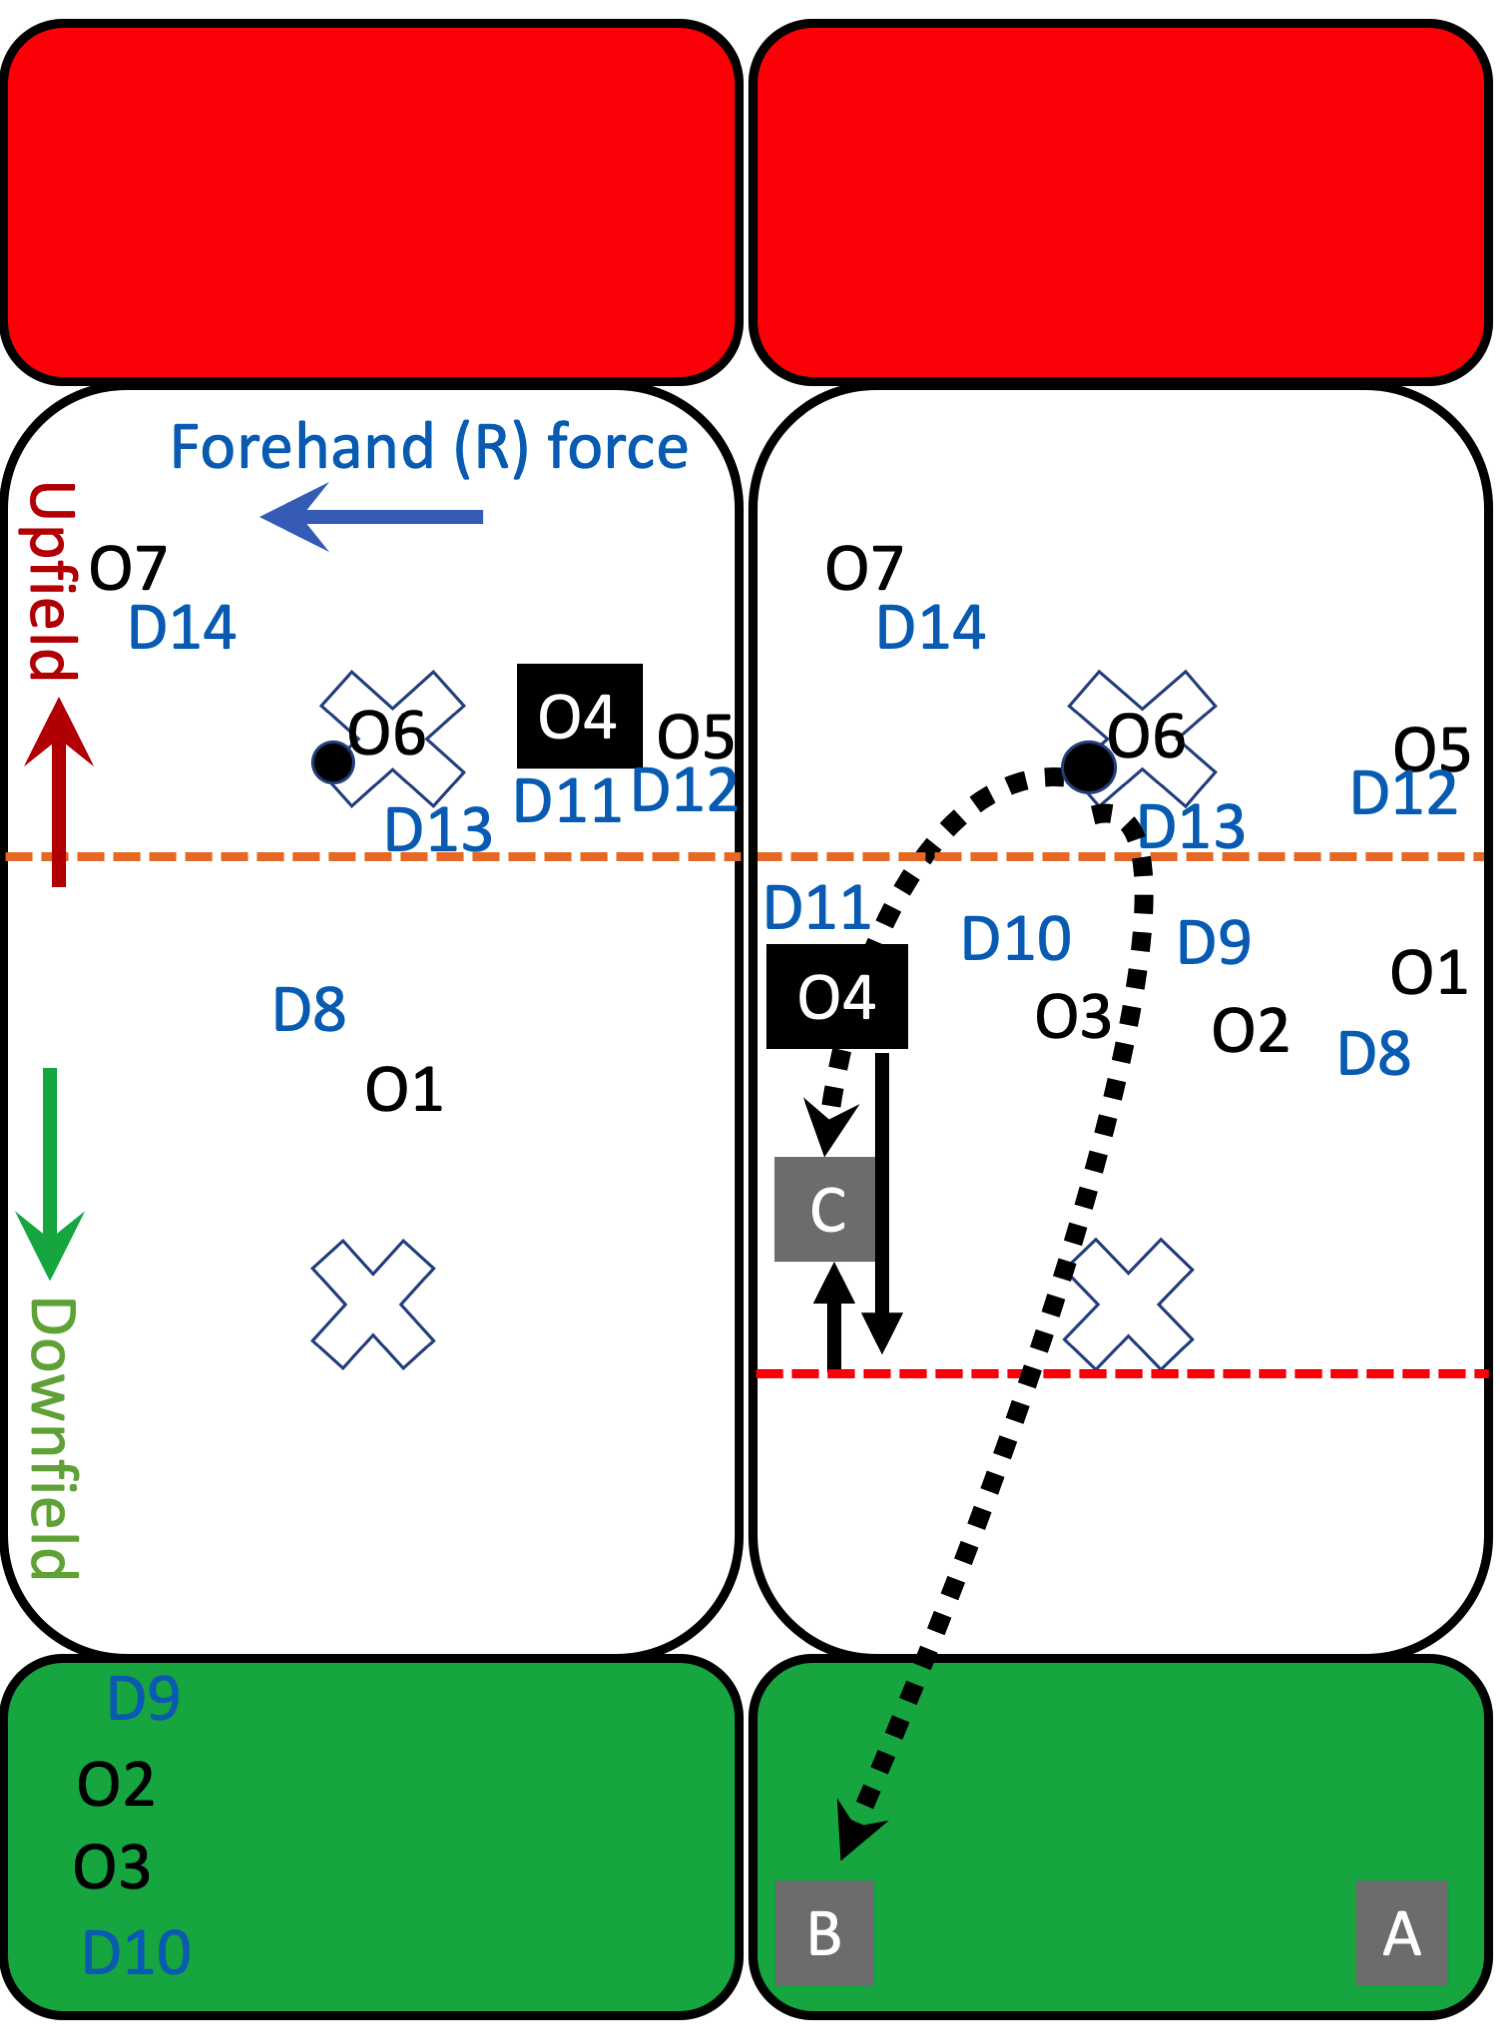
\includegraphics[width=\linewidth]{O4-horizontal}
  \caption{Feld (left) \& ho-ro (right)}
  \label{fig:O4-horizontal}
\end{marginfigure}

It may be that 
one of 
D9 
and D10 
go to help D8 
cover D1.  
If so, 
you and O2 
might spread out, 
one on each side line,
and move a bit closer, 
so as to receive a pass from 
the handlers directly.  


\subsection{Beating person-match defence with a horizontal stack}\label{sec:horizontall}
Horizontal stack 
typically involves cutting
upfield and downfield (black arrows)
within your quarter of the field\footnote{
Other cuts
can work, 
but might need
communication,
e.g. diamond cuts 
involve trading places 
with O1 
or O4.}
as shown in 
Figure \ref{fig:O4-horizontal}(right).
O6 
can potentially 
throw to you 
in the endzone 
or at C\footnote{
Black arrows
show how a back-under cut 
opens space 
for the throw 
to C.}. 

\section{Beating zone defence}\label{sec:zone}
\begin{marginfigure}%
  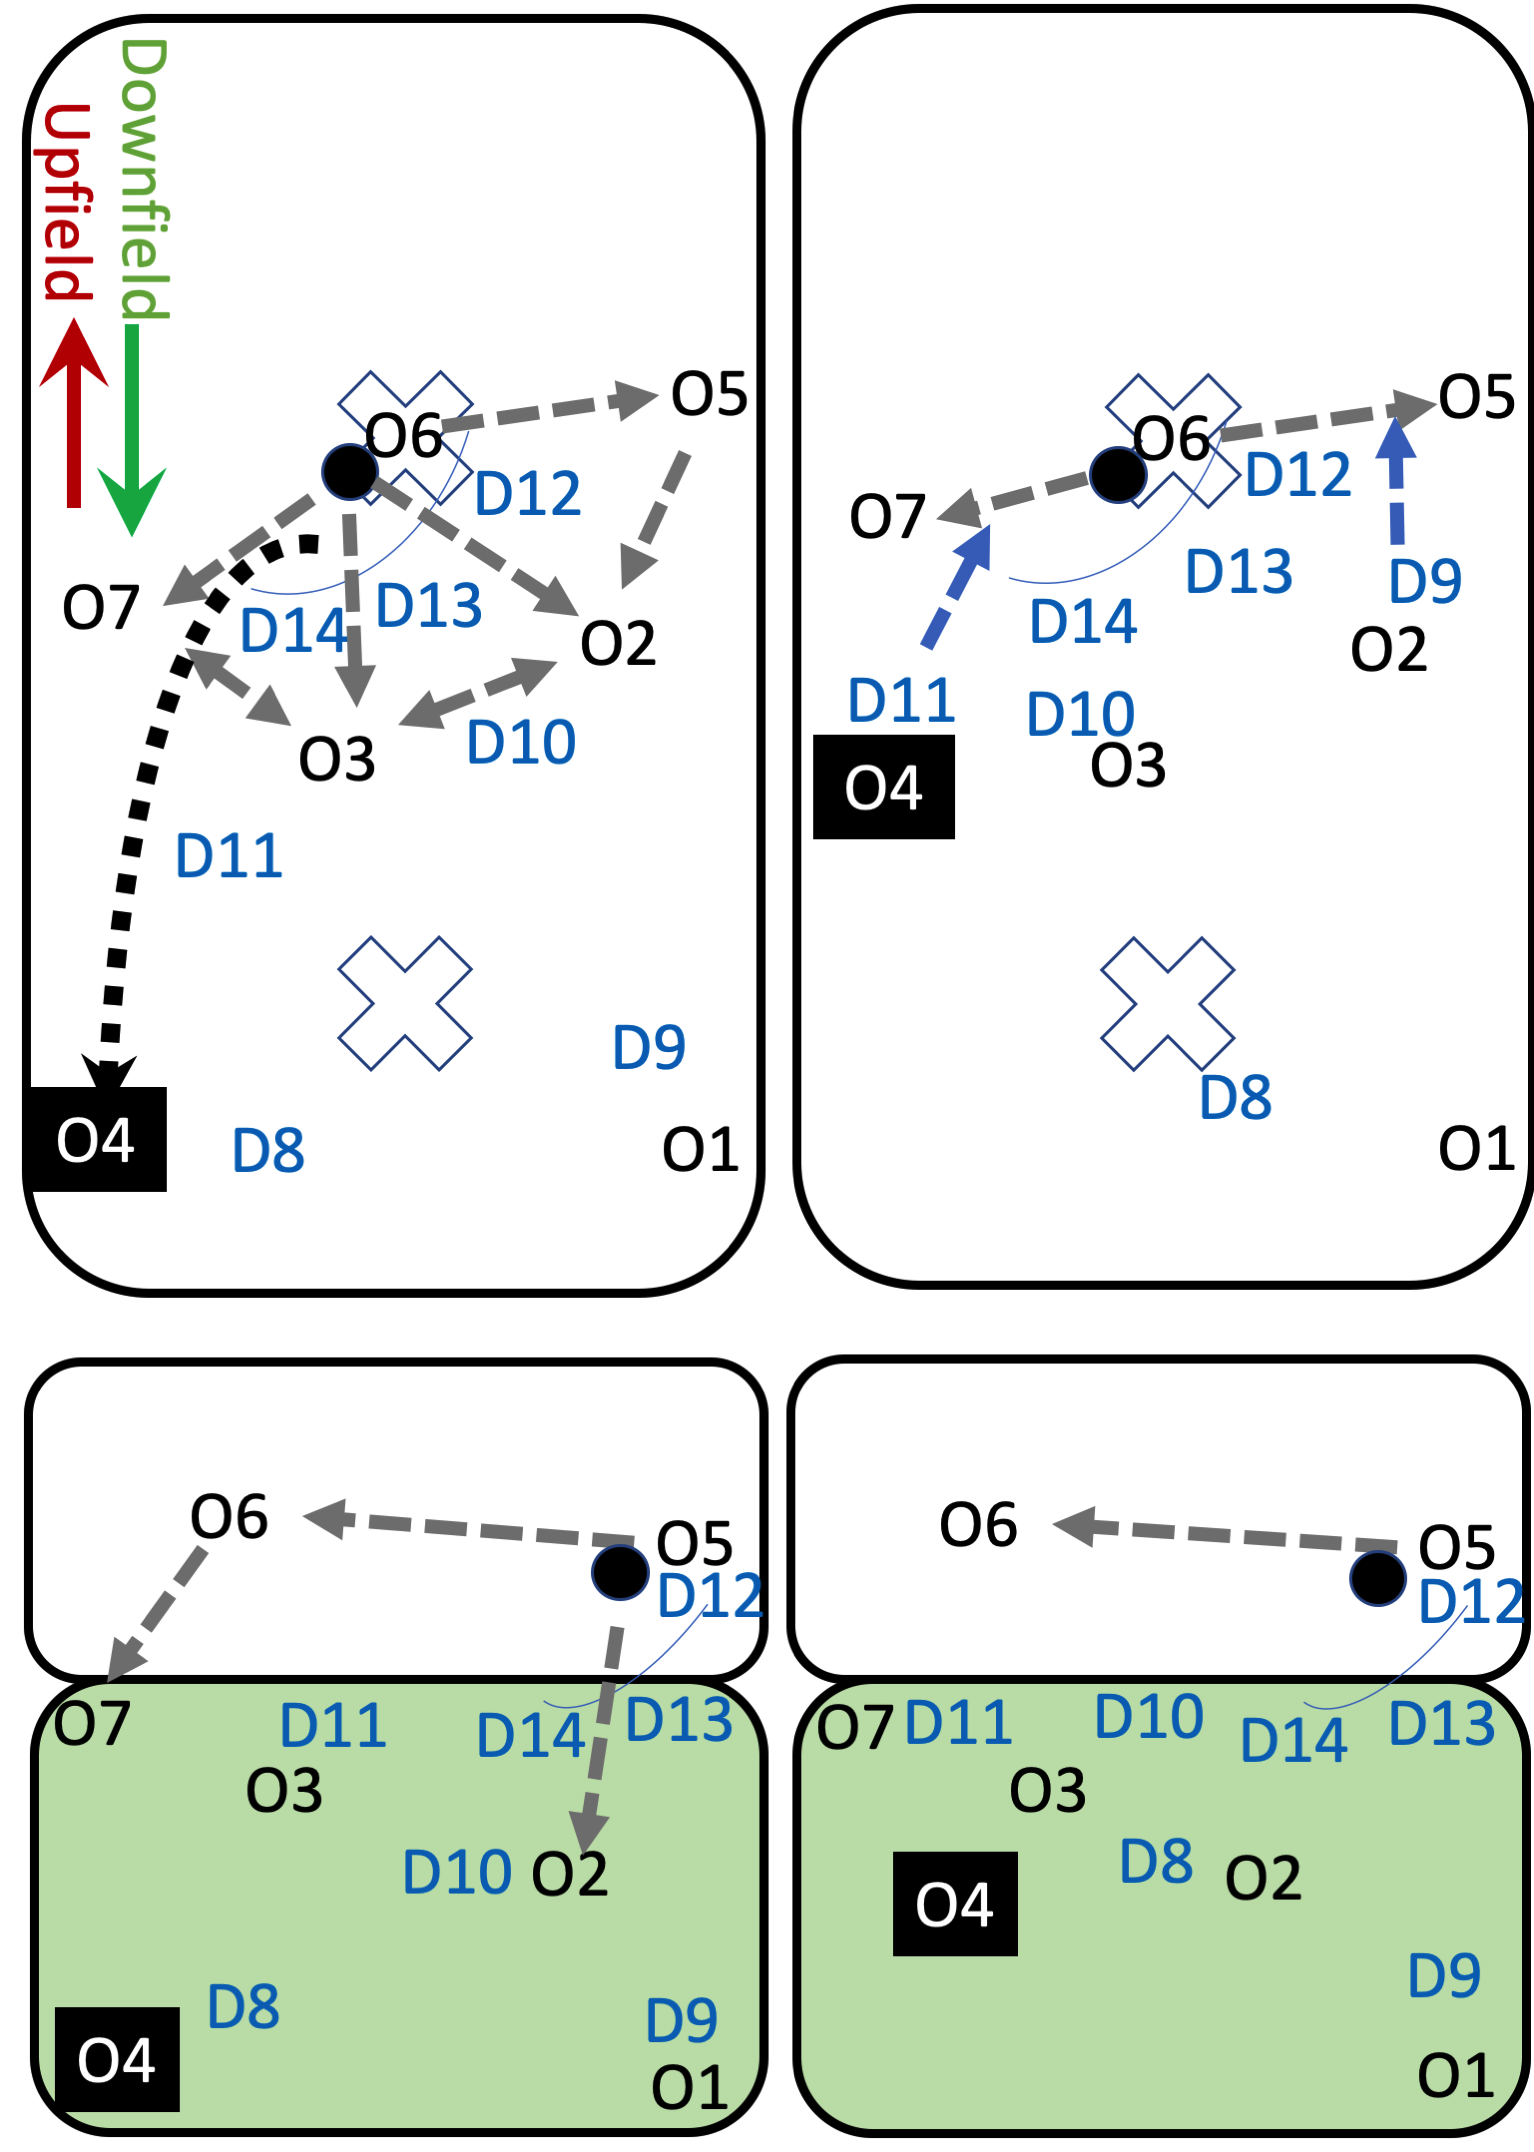
\includegraphics[width=\linewidth]{O4-zone331}
  \caption{formations against 331 zone}
  \label{fig:O4-zone331}
\end{marginfigure}
Vertical stack 
probably won't work
against zone. 
Instead, your 
team might do better spreading out, 
as shown 
in Figure \ref{fig:O4-zone331}. 
Three ways to beat a zone are:
(1) over;
(2) round; or
(3) through. 
Figure \ref{fig:O4-zone331}
(top left)
shows this 
with you 
behind the cup, 
potentially receiving a pass 
\smallcaps{through} 
between 
D13 
and D14, or 
\smallcaps{over} 
the cup\footnote{
Short hammer, scoober.}.
Alternatively, 
it might go 
\smallcaps{round} 
to O7 then 
\smallcaps{further round} to you.

Also to consider
is how you 
coordinate 
with O2 
to split 
D10. 
Figure \ref{fig:O4-zone331}
(top left), 
shows D10 
having to 
cover both 
you and O2, 
maybe with help 
from D9 
and D11. 
In contrast, 
Figure \ref{fig:O4-zone331}
(top right) 
shows a position 
that might occur 
if you `crash' 
the cup\footnote{ 
Crashing 
might  
disrupt the 
cup's formation and 
allow a stall reset.  
But, I'm not a huge fan, 
unless its a handlers 
crashing from behind, 
because you lose 
a player downfield},
which allows
D10 
to ignore you 
and play 
tighter on O2\footnote{ 
It might also allow 
D11 to threaten to intercept 
a pass to O7, 
and the rest of the cup 
(D12-13) 
to do more 
to block throws 
to O2 or O5. 
In general, 
crashing the cup
changes 
the downfield situation 
to 3 (O1, O2 and O4) 
versus 4 (D8-11), 
which is not ideal.}. 
Figure \ref{fig:O4-zone331}hat
(bottom left and right)
show two possible 
positions close to the 
endzone. 
Again, as O4
your role might 
be to try 
and work with 
O2, O5 and O7 
such that D10 
and D11 are unable to 
cover you all.   


\section{Beating clam defence}\label{sec:zone}
Clam mixes person-match 
and zone defence styles, 
with defenders 
switching frequently.
%\footnote{
%For example, 
%in Figure \ref{fig:O4-vertical}(left) 
%D8 
%might cover 
%O1 deep, 
%switching later 
%(with D9 or D11
%to cover O4's cut deep,
%rather than following O1 
%upfield to C.}. 
You might
coordinate 
with others  
to overload 
a defender, 
or spread out 
and give the handlers 
space 
and targets deep. 

\newthought{...and finally} 
this is just a two pager; 
there are many more 
offensive strategies 
and tactics\footnote{
Try no formation, just a string: O1-throws-to-O2-who-throws-to-O4-etc. Bonus points for getting all the way to O7 before scoring!}
Remember, 
defence wins games, 
offence loses them\footnote{
Because the team with the least turnovers 
usually wins.};.
and it's better to get it back 
with another turnover\footnote{
i.e. if you offence fails, then its time to play defence, even though you're the O team :)}
than receiving another pull!

\end{document}
